\documentclass[tikz,border=10pt]{standalone}
% Only base TikZ is needed; no extra libraries.
\begin{document}
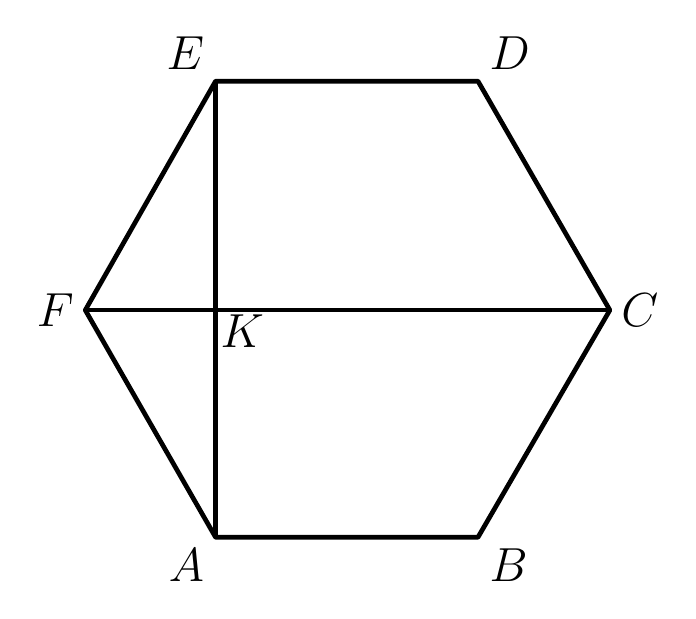
\begin{tikzpicture}[line join=round, line width=1.7pt]
  % Vertices: GES units (1 unit = 100 px) scaled by 2.122 cm per unit (metrics scale 0.02122 cm/px * 100 px)
  \coordinate (E) at (3.119,-1.379);
  \coordinate (D) at (6.451,-1.379);
  \coordinate (C) at (8.126,-4.287);
  \coordinate (B) at (6.451,-7.172);
  \coordinate (A) at (3.119,-7.172);
  \coordinate (F) at (1.464,-4.287);
  \coordinate (K) at (3.119,-4.287);

  % Hexagon outline
  \draw (E) -- (D) -- (C) -- (B) -- (A) -- (F) -- cycle;

  % Interior segments through K
  \draw (F) -- (C);
  \draw (E) -- (A);

  % Labels
  \node[above left] at (E) {\fontsize{17}{20.4}\selectfont $E$};
  \node[above right] at (D) {\fontsize{17}{20.4}\selectfont $D$};
  \node[right] at (C) {\fontsize{17}{20.4}\selectfont $C$};
  \node[below right] at (B) {\fontsize{17}{20.4}\selectfont $B$};
  \node[below left] at (A) {\fontsize{17}{20.4}\selectfont $A$};
  \node[left] at (F) {\fontsize{17}{20.4}\selectfont $F$};
  \node[below right, inner sep=1pt] at (K) {\fontsize{17}{20.4}\selectfont $K$};
\end{tikzpicture}
\end{document}